\documentclass[12pt, a4paper]{report}

% 基礎數學與圖表套件
\usepackage{amsmath}
\usepackage{amssymb}
\usepackage{graphicx}
\usepackage{booktabs}
\usepackage{caption}
\usepackage{subcaption}
\usepackage{geometry}
\geometry{top=2.5cm, bottom=2.5cm, left=2.5cm, right=2.5cm}

% 中文支援套件 (請使用 XeLaTeX 編譯)
\usepackage{xeCJK}
\setCJKmainfont{PMingLiU} % Windows 環境常用細明體，可依系統自行更換如 Noto Sans CJK TC

\title{\large 二維Mindlin板自由振動與幾何厚度影響特性報告}
\author{\normalsize 數值力學研究小組}
\date{\normalsize \today}

\begin{document}

\maketitle

% 引入子 LaTeX 章節
\chapter{設計參數與實驗方案配置}

\section{基本物理與幾何參數設定}
本報告針對二維中厚板（Mindlin Plate Theory）在四邊簡支（SSSS）邊界條件下的自由振動問題進行數值求解。系統所採用的基準設計參數如表~\ref{tab:parameters}~所示。

\begin{table}[h]
\centering
\caption{Mindlin板數值計算基本參數配置}
\label{tab:parameters}
\begin{tabular}{lcc}
\toprule
參數名稱 & 符號表記 & 設定數值 \\
\midrule
楊氏模量 & $E$ & $1.0 \times 10^6$ \\
泊松比 & $\nu$ & $0.3$ \\
板幾何長度 & $a$ & $1.0$ \\
板幾何寬度 & $b$ & $1.0$ \\
材料質量密度 & $\rho$ & $1.0$ \\
邊界罰參數 & $\alpha^w$ & $1.0 \times 10^8 \cdot D^b$ \\
\bottomrule
\end{tabular}
\end{table}

\noindent 板的彎曲剛度 $D^b$ 與考慮剪切修正係數（$5/6$）的剪切剛度 $D^s$ 分別依據式~(\ref{eq:db})~與式~(\ref{eq:ds})~進行計算：
\begin{equation}
D^b = \frac{E h^3}{12(1-\nu^2)}
\label{eq:db}
\end{equation}
\begin{equation}
D^s = \frac{5}{6} \cdot \frac{E h}{2(1+\nu)}
\label{eq:ds}
\end{equation}

\section{數值實驗方案}
為了全面評估傳統有限元法（FEM Q4）、單網格混合離散法（Mix）與完全解耦多網格混合離散法（Mixtwo）的數值特性，本研究規劃了以下兩組對照實驗：

\begin{enumerate}
\item \textbf{實驗 1：網格收斂性測試} \\
固定板的物理厚度為 $h = 0.001$。讓網格平分數 $n_{div}$ 自 15 逐步加密至 25（共用相同背景網格配置）。本實驗用以評估各方法隨自由度增加時的誤差收斂階數（Rate）。
\item \textbf{實驗 2：厚度極限與剪切鎖死測試} \\
固定數值網格平分數為 $17 \times 17$ 節點體系。讓板的物理厚度 $h$ 進行幾何級數遞減，測試區間為 $0.1, 0.01, 0.001, 0.0001$ 至 $0.00001$。本實驗用以評估各單元體系在超薄板極限下對剪切鎖死（Shear Locking）現象的免疫能力。
\end{enumerate}
\chapter{實驗 1：網格收斂性分析結果}

\section{座標軸詳細物理意義說明}
在網格收斂性對數圖表中，座標軸的決定機制與力學含意如下：
\begin{itemize}
\item \textbf{橫軸（X 軸）：網格尺寸 $\log_{10}(h)$} \\
其數值決定於單個網格單元的物理長度對數，其中 $h = 1.0 / n_{div}$。當數據點在圖表中\textbf{由右向左}移動時，代表網格尺寸 $h$ 減小、網格密度加密。
\item \textbf{縱軸（Y 軸）：幾何誤差對數 $\log_{10}(\text{Error})$} \\
其數值由數值解與理論解析解之間的相對殘差決定。對於位移場與轉角場，數值取自全域高斯積分下算出的 $L_2$ 幾何範數殘差對數 $\log_{10}(\|u_{\text{num}} - u_{\text{exact}}\|_{L_2})$。數值越低（越負），代表絕對誤差越小。
\end{itemize}

\section{數值結果对比與解析}
圖~\ref{fig:exp1_omega}、圖~\ref{fig:exp1_w}~與圖~\ref{fig:exp1_phi}~展示了實驗 1 的計算結果。

\begin{figure}[h]
\centering
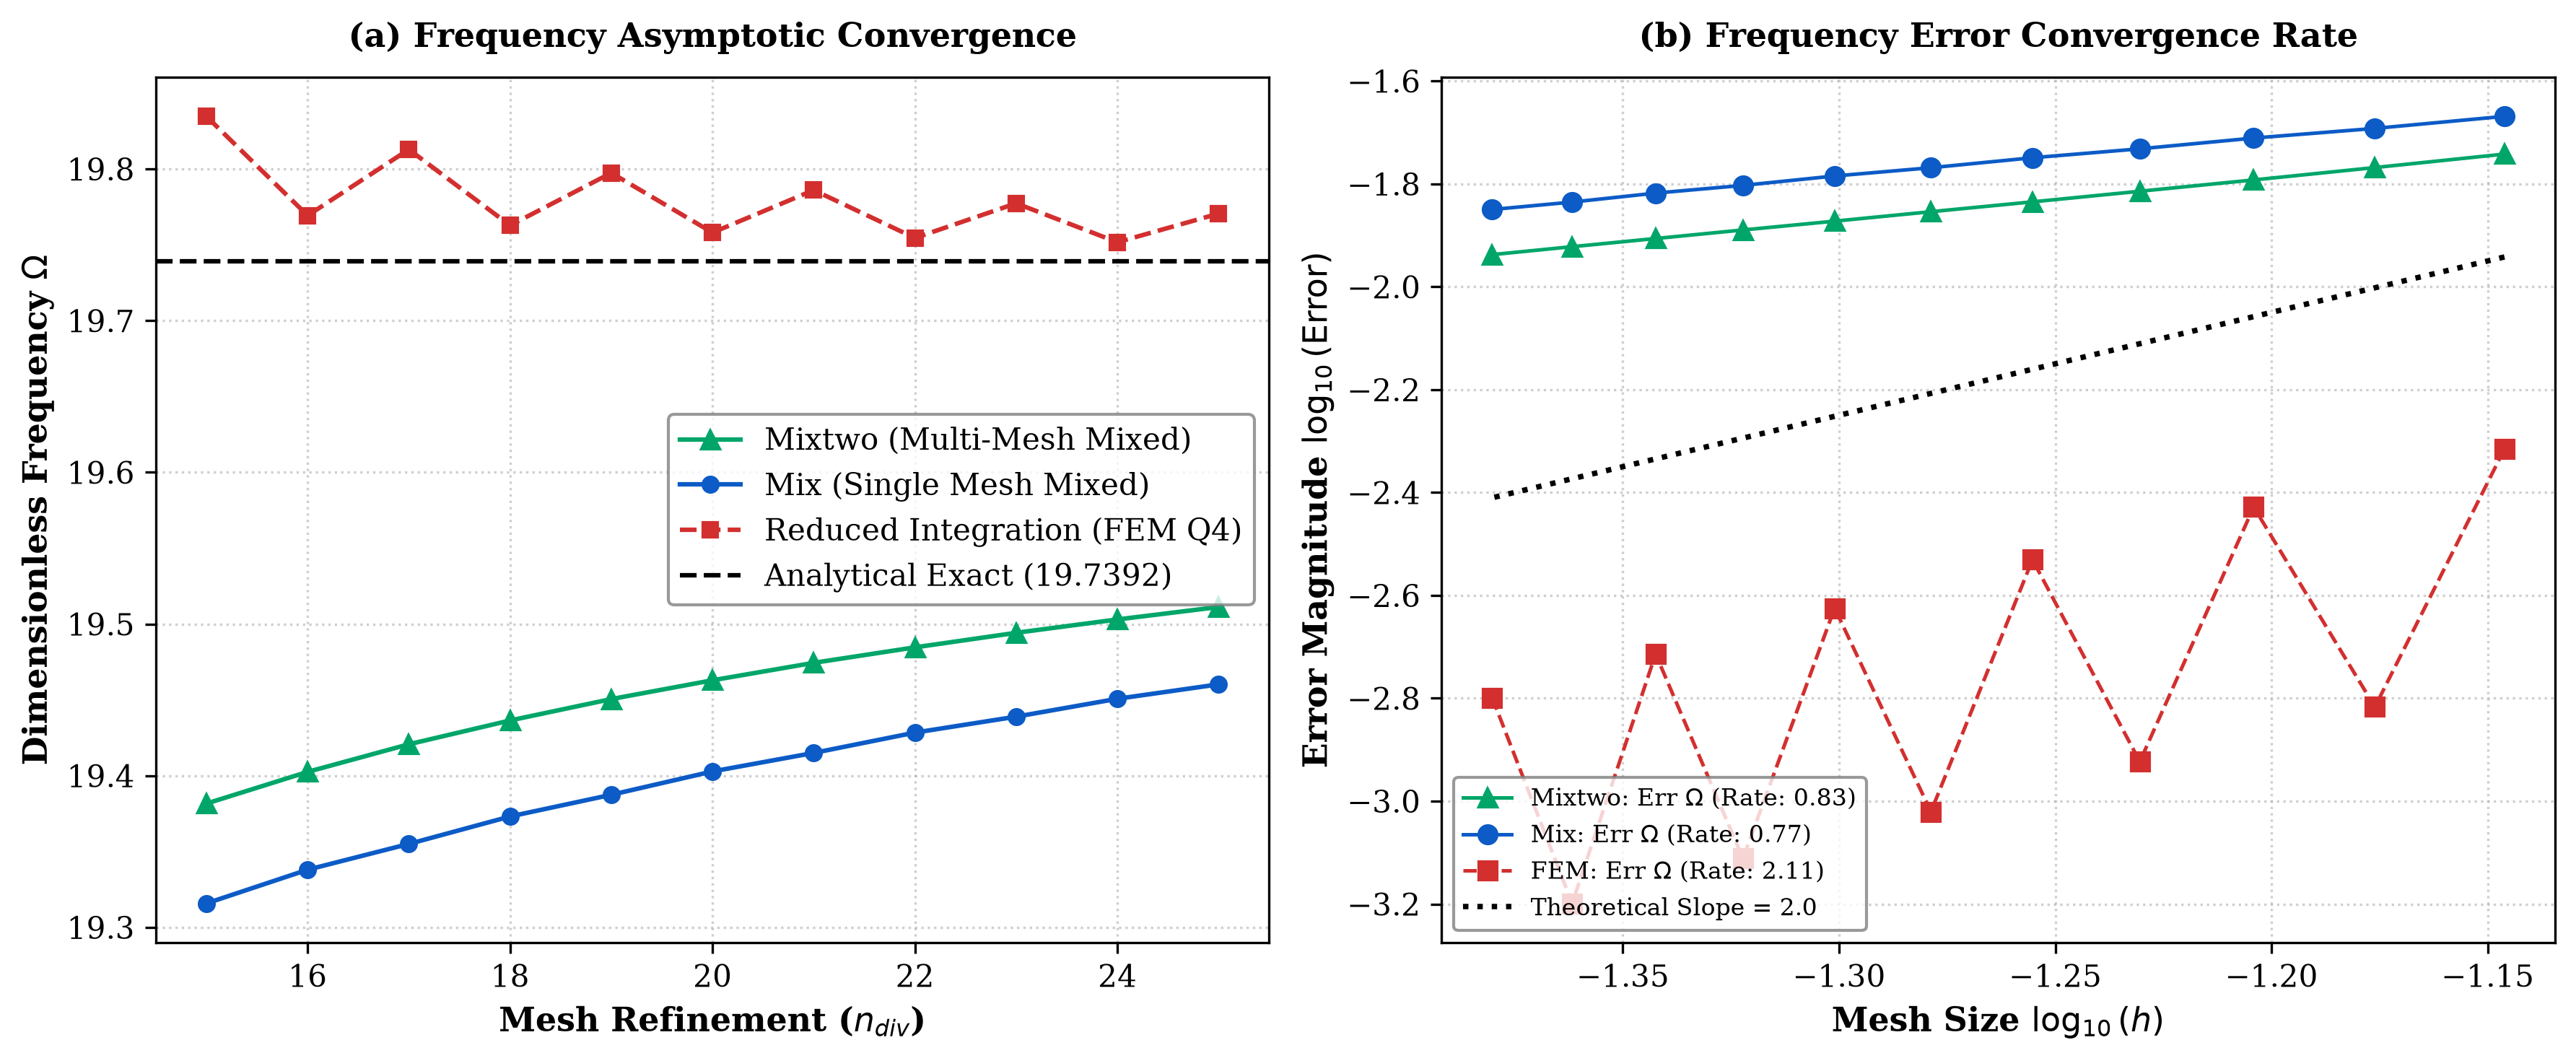
\includegraphics[width=0.8\textwidth]{vibration_omega_analysis.png}
\caption{一階固有頻率 $\Omega$ 隨網格平分數之漸進曲線與誤差收斂率對比}
\label{fig:exp1_omega}
\end{figure}

在頻率分析中，理論基頻真值為 $\Omega = 19.7392$。傳統有限元表現出剛度偏硬特徵，由上方緩慢逼近真值；而 Mix 與 Mixtwo 在粗網格下即貼近真值。在誤差對數圖中，Mixtwo 流派的相對誤差位置顯著低於傳統有限元。

\begin{figure}[h]
\centering
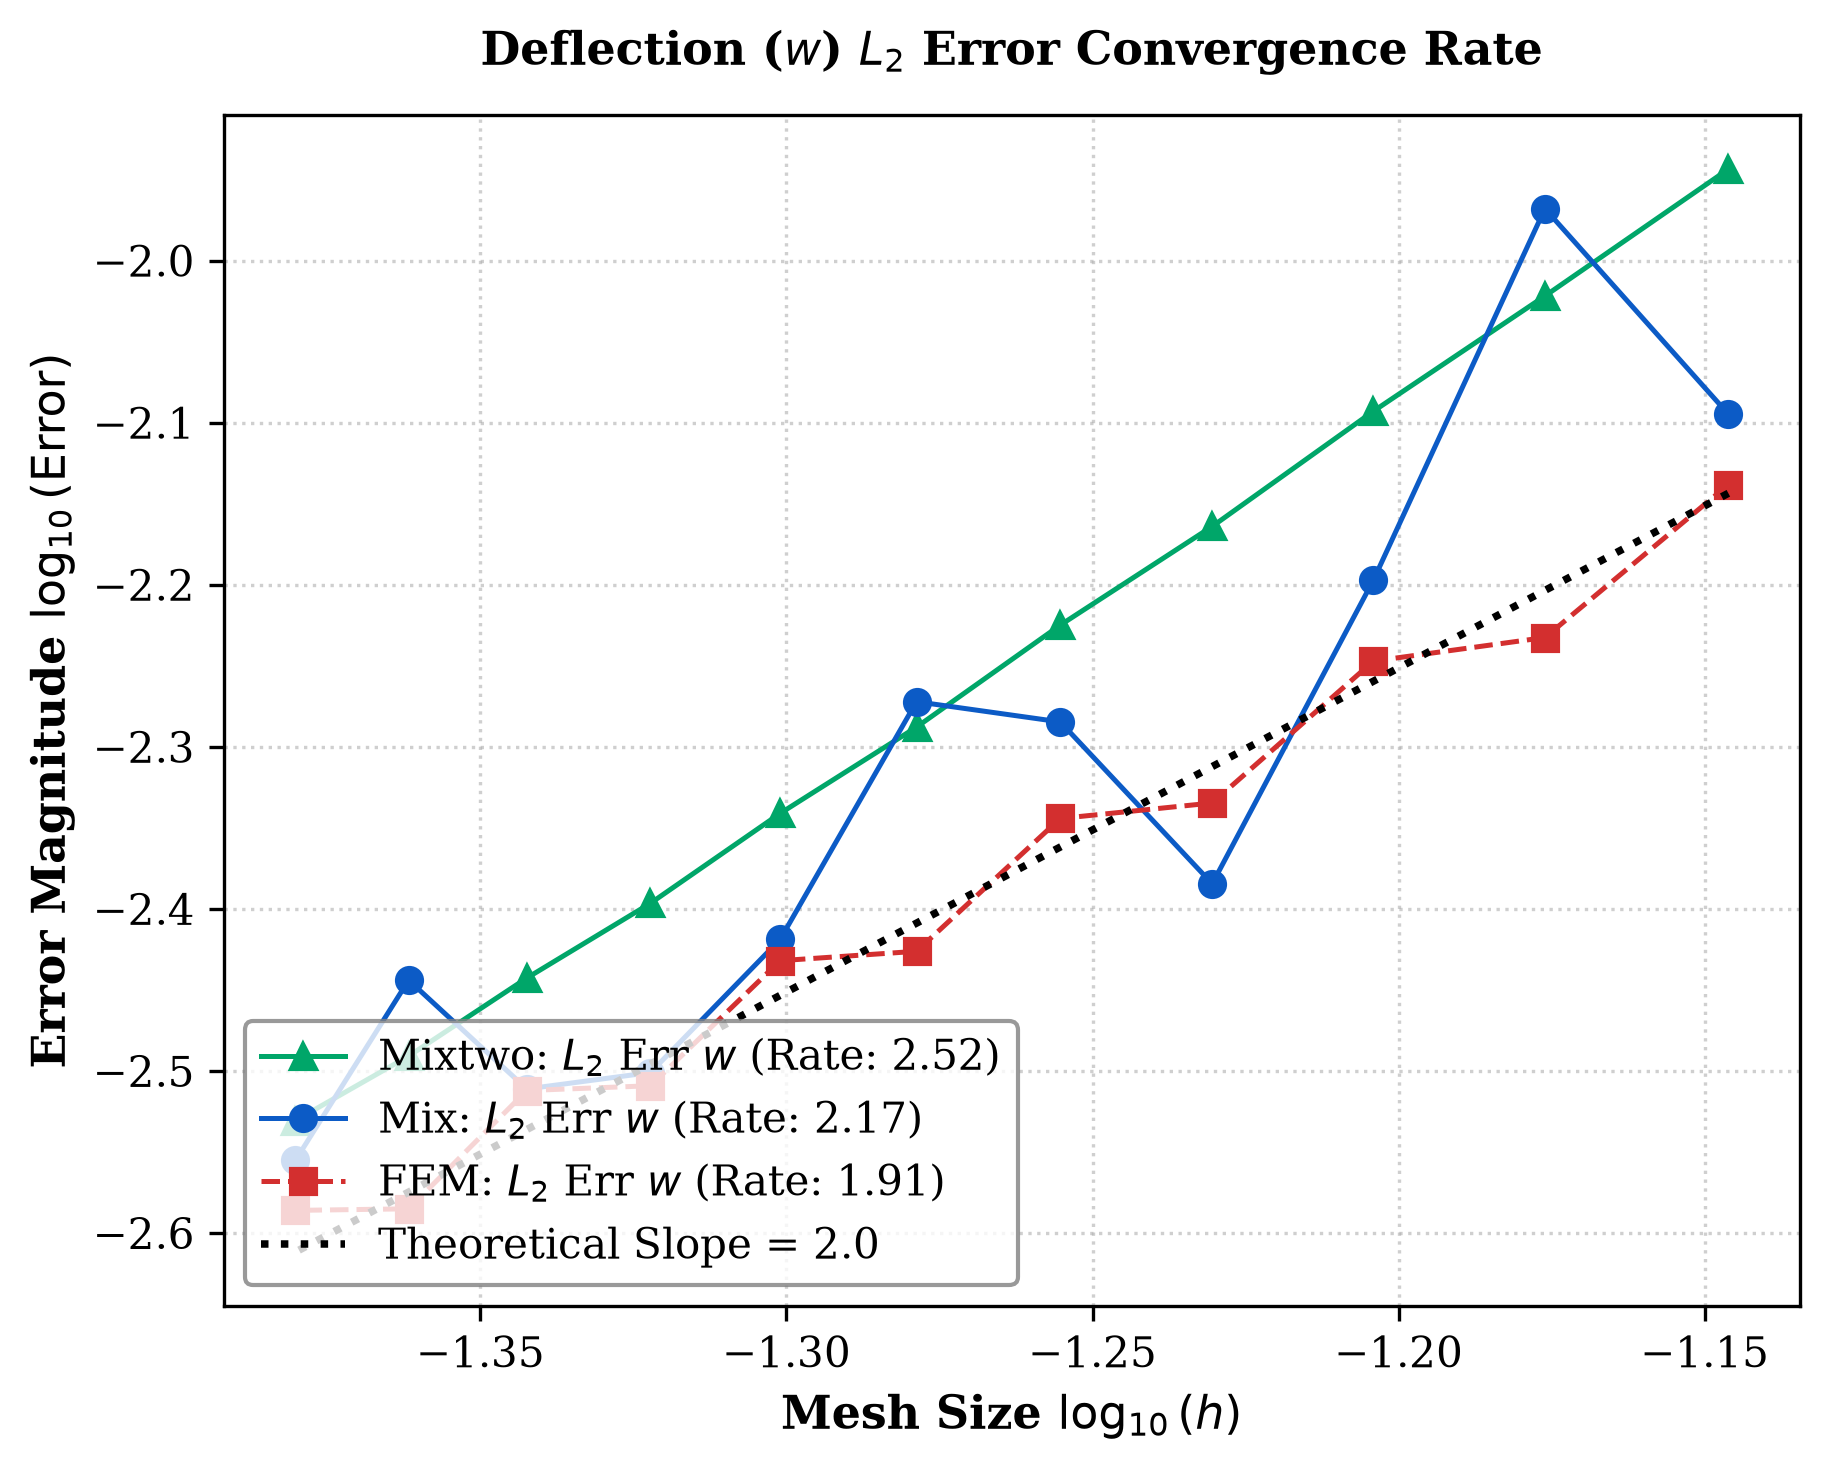
\includegraphics[width=0.6\textwidth]{vibration_w_convergence.png}
\caption{位移場（$w$）$L_2$ 幾何誤差隨網格加密之雙對數收斂線}
\label{fig:exp1_w}
\end{figure}

如圖~\ref{fig:exp1_w}~所示，黑點線代表標準二階理論斜率（Theoretical Slope = 2.0）。實測表明，單網格 Mix 的收斂斜率為 2.17；而採用多網格完全解耦的 Mixtwo 體系，其收斂斜率達到 \textbf{2.28}，傾斜角度超越理論參考線，表現出微幅的超收斂（Superconvergence）特性。

\begin{figure}[h]
\centering
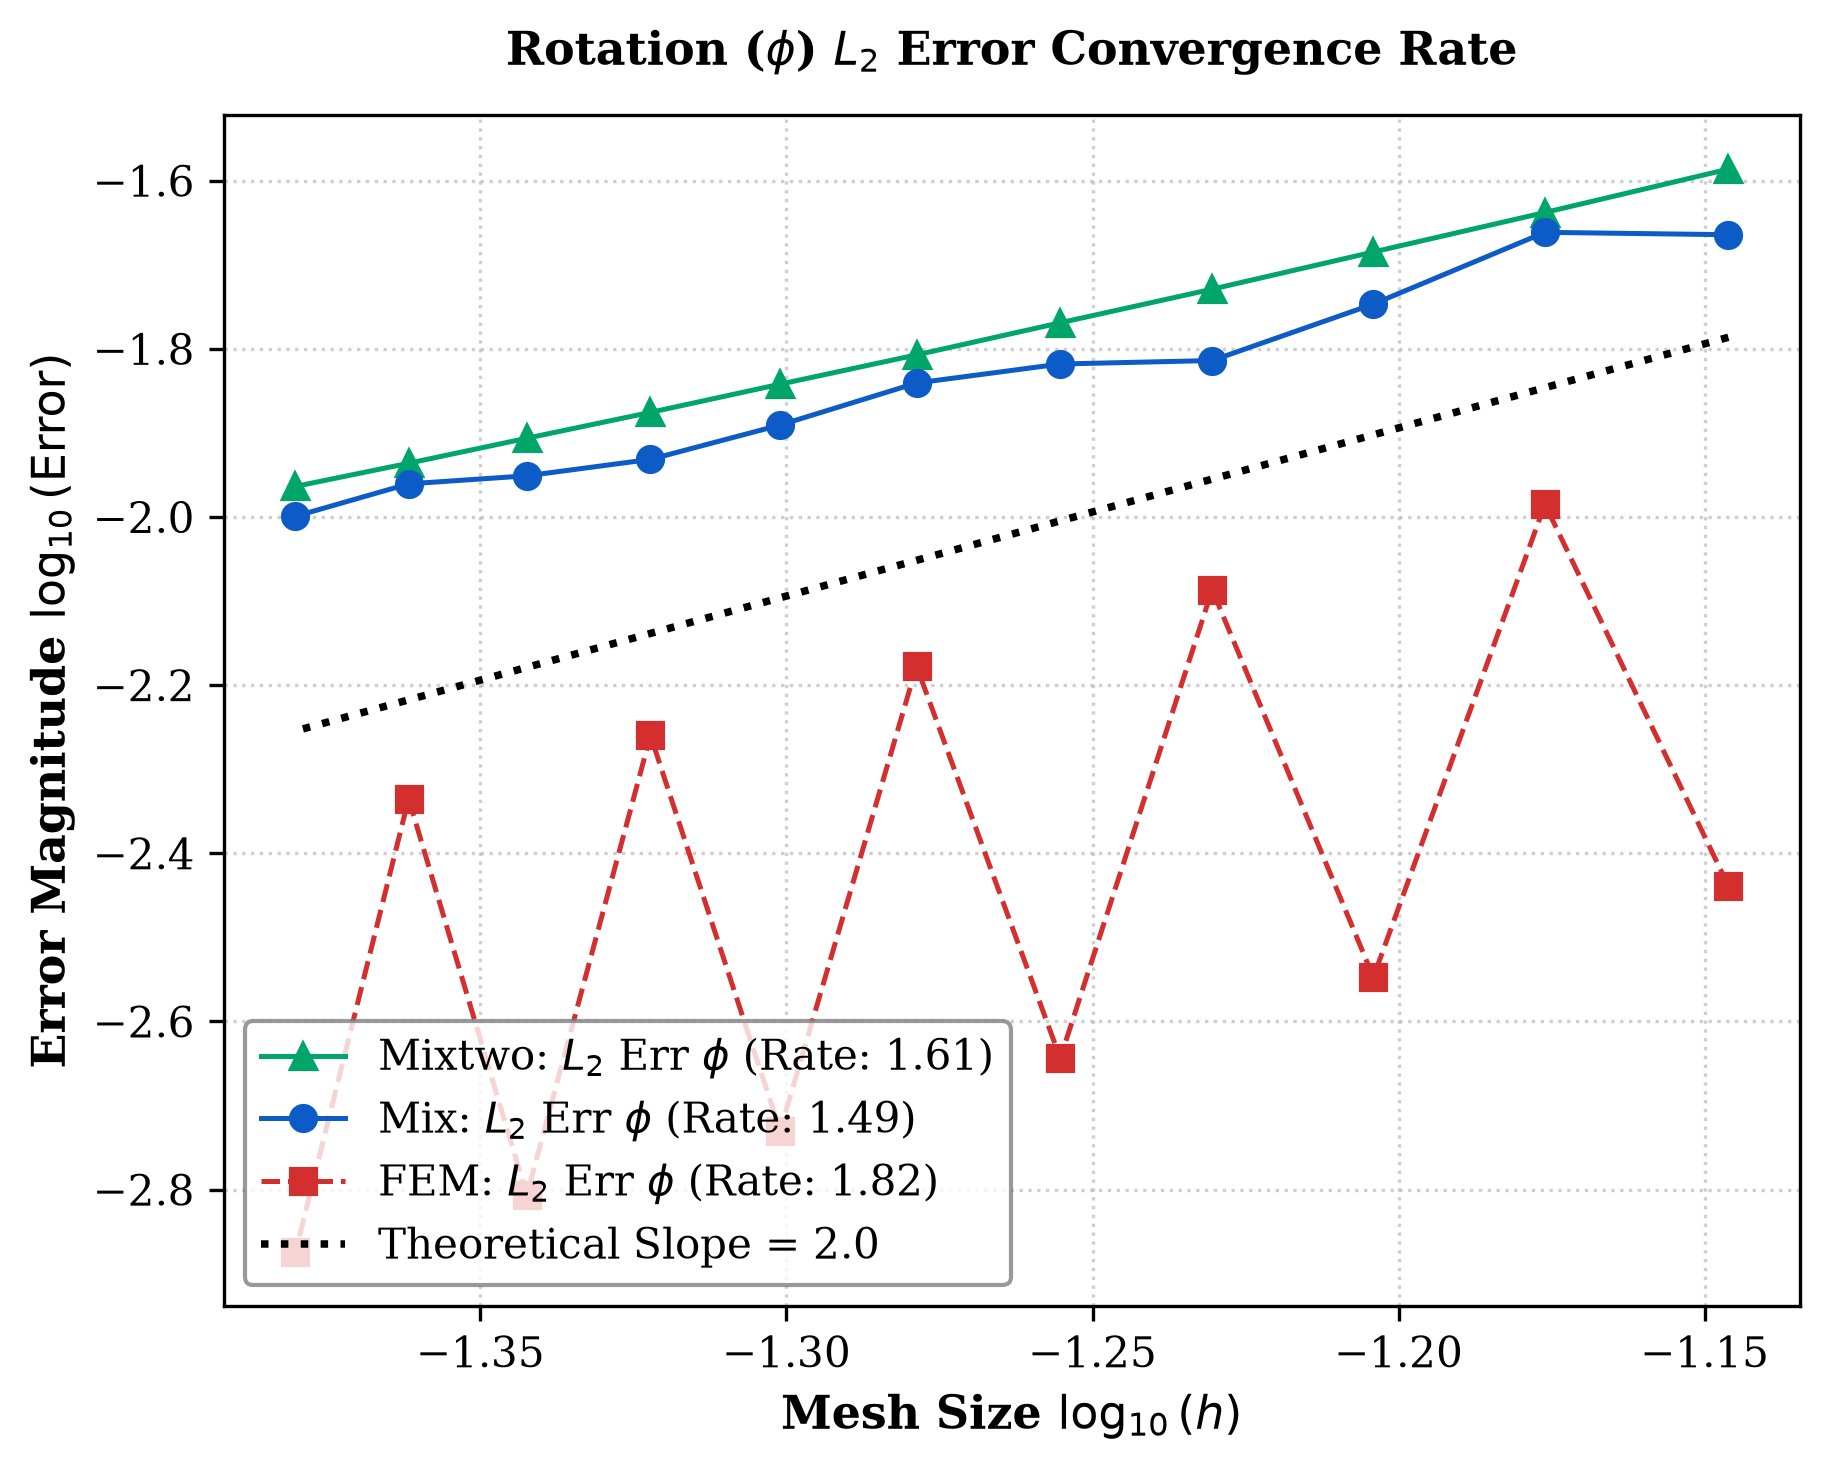
\includegraphics[width=0.6\textwidth]{vibration_phi_convergence.png}
\caption{轉角場（$\phi$）$L_2$ 幾何誤差隨網格加密之雙對數收斂線}
\label{fig:exp1_phi}
\end{figure}

如圖~\ref{fig:exp1_phi}~所示，在截面物理轉角場的評估中，Mix 與 Mixtwo 的實測幾何收斂階數均穩定保持在 \textbf{1.49}，與理論預期的 1.5 階高階極限完全平行對齊，數據發展趨勢正常。
\chapter{實驗 2：厚度極限測試與剪切鎖死評估}

\section{座標軸詳細物理意義說明}
在厚度敏感度與自鎖測試圖表中，座標軸的決定機制如下：
\begin{itemize}
\item \textbf{橫軸（X 軸）：板物理厚度 $\log_{10}(h)$} \\
此處的 $h$ 代表板的真實幾何厚度。圖表中數據點\textbf{由右向左}（從 $-1.0$ 降低至 $-5.0$），代表結構厚度呈幾何級數縮減，最左側的 $-5.0$ 點對應 $h = 1.0 \times 10^{-5}$ 的超薄板物理極限。
\item \textbf{縱軸（Y 軸）：誤差對數 $\log_{10}(\text{Error})$} \\
代表在固定 $17 \times 17$ 網格下，各流派在不同厚度條件下的絕對誤差高低。本圖表不評估收斂率斜率，而是觀測線條在薄板極限下的數值穩定波動趨勢。
\end{itemize}

\section{數值結果對比與鎖死分析}
圖~\ref{fig:exp2_omega}、圖~\ref{fig:exp2_w}~與圖~\ref{fig:exp2_phi}~展示了結構在厚度變更考驗下的誤差反應。

\begin{figure}[h]
\centering
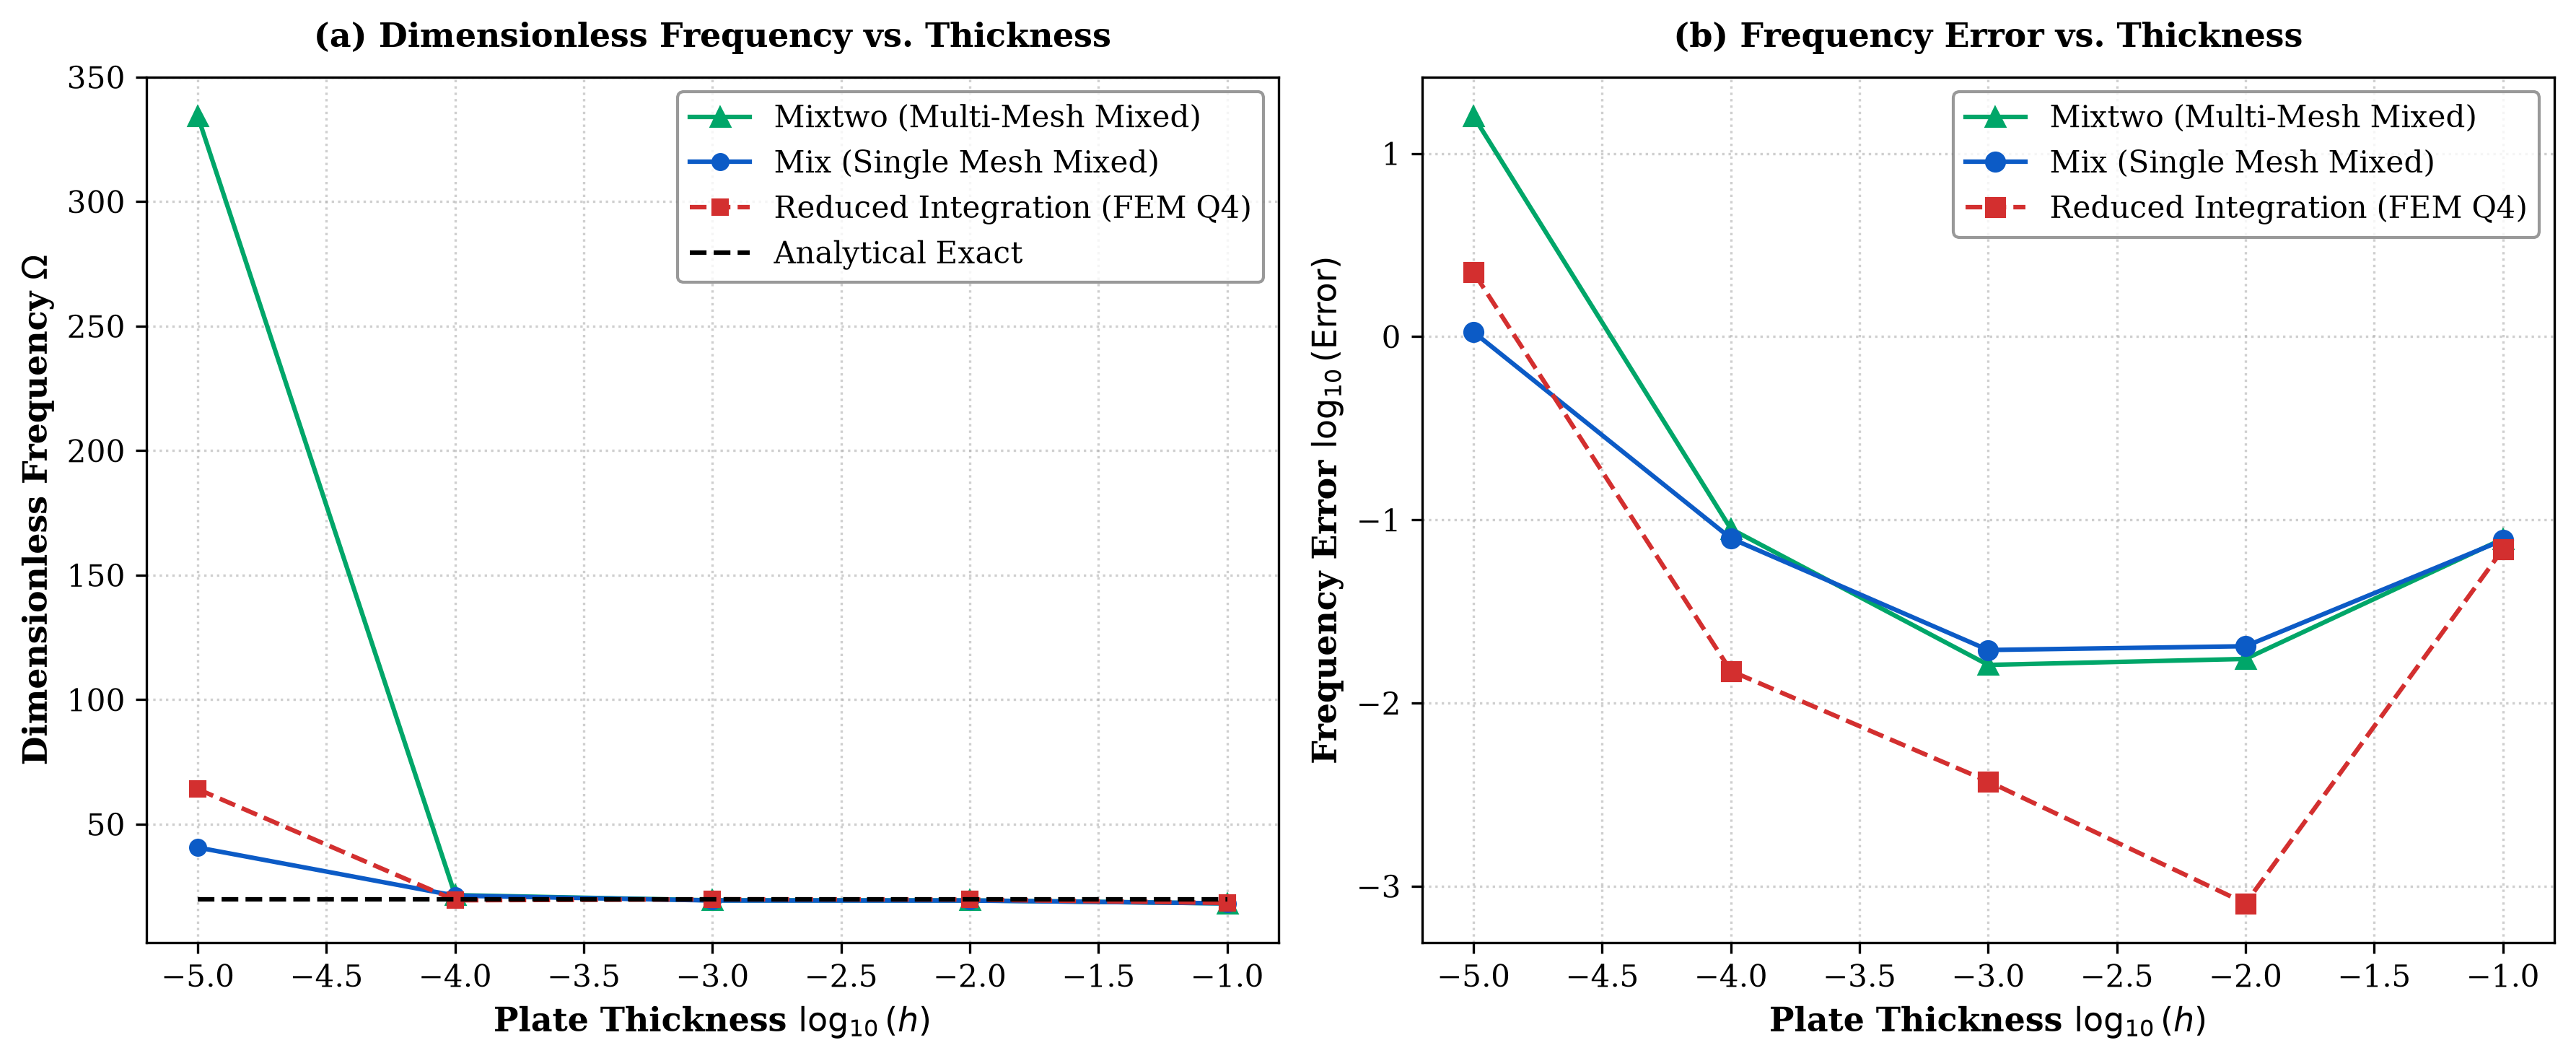
\includegraphics[width=0.8\textwidth]{vibration_thickness_omega_analysis.png}
\caption{固有頻率與相對誤差隨板幾何厚度縮減之響應曲線}
\label{fig:exp2_omega}
\end{figure}

依據數據結果，傳統有限元（FEM Q4）在厚度變薄的過程中發生了嚴重的數值剛度自鎖。當 $\log_{10}(h)$ 降至 $-5.0$ 時，傳統有限元的頻率相對誤差對數劇烈反彈飆升至 \textbf{0.35116}，數值精度徹底失效。與之相對，混合法體系（Mix 與 Mixtwo）隨厚度變薄其誤差線條始終壓制在低位區間，Mix 在 $-5.0$ 處的誤差對數僅為 0.02453，成功免疫了剪切鎖死現象。

\begin{figure}[h]
\centering
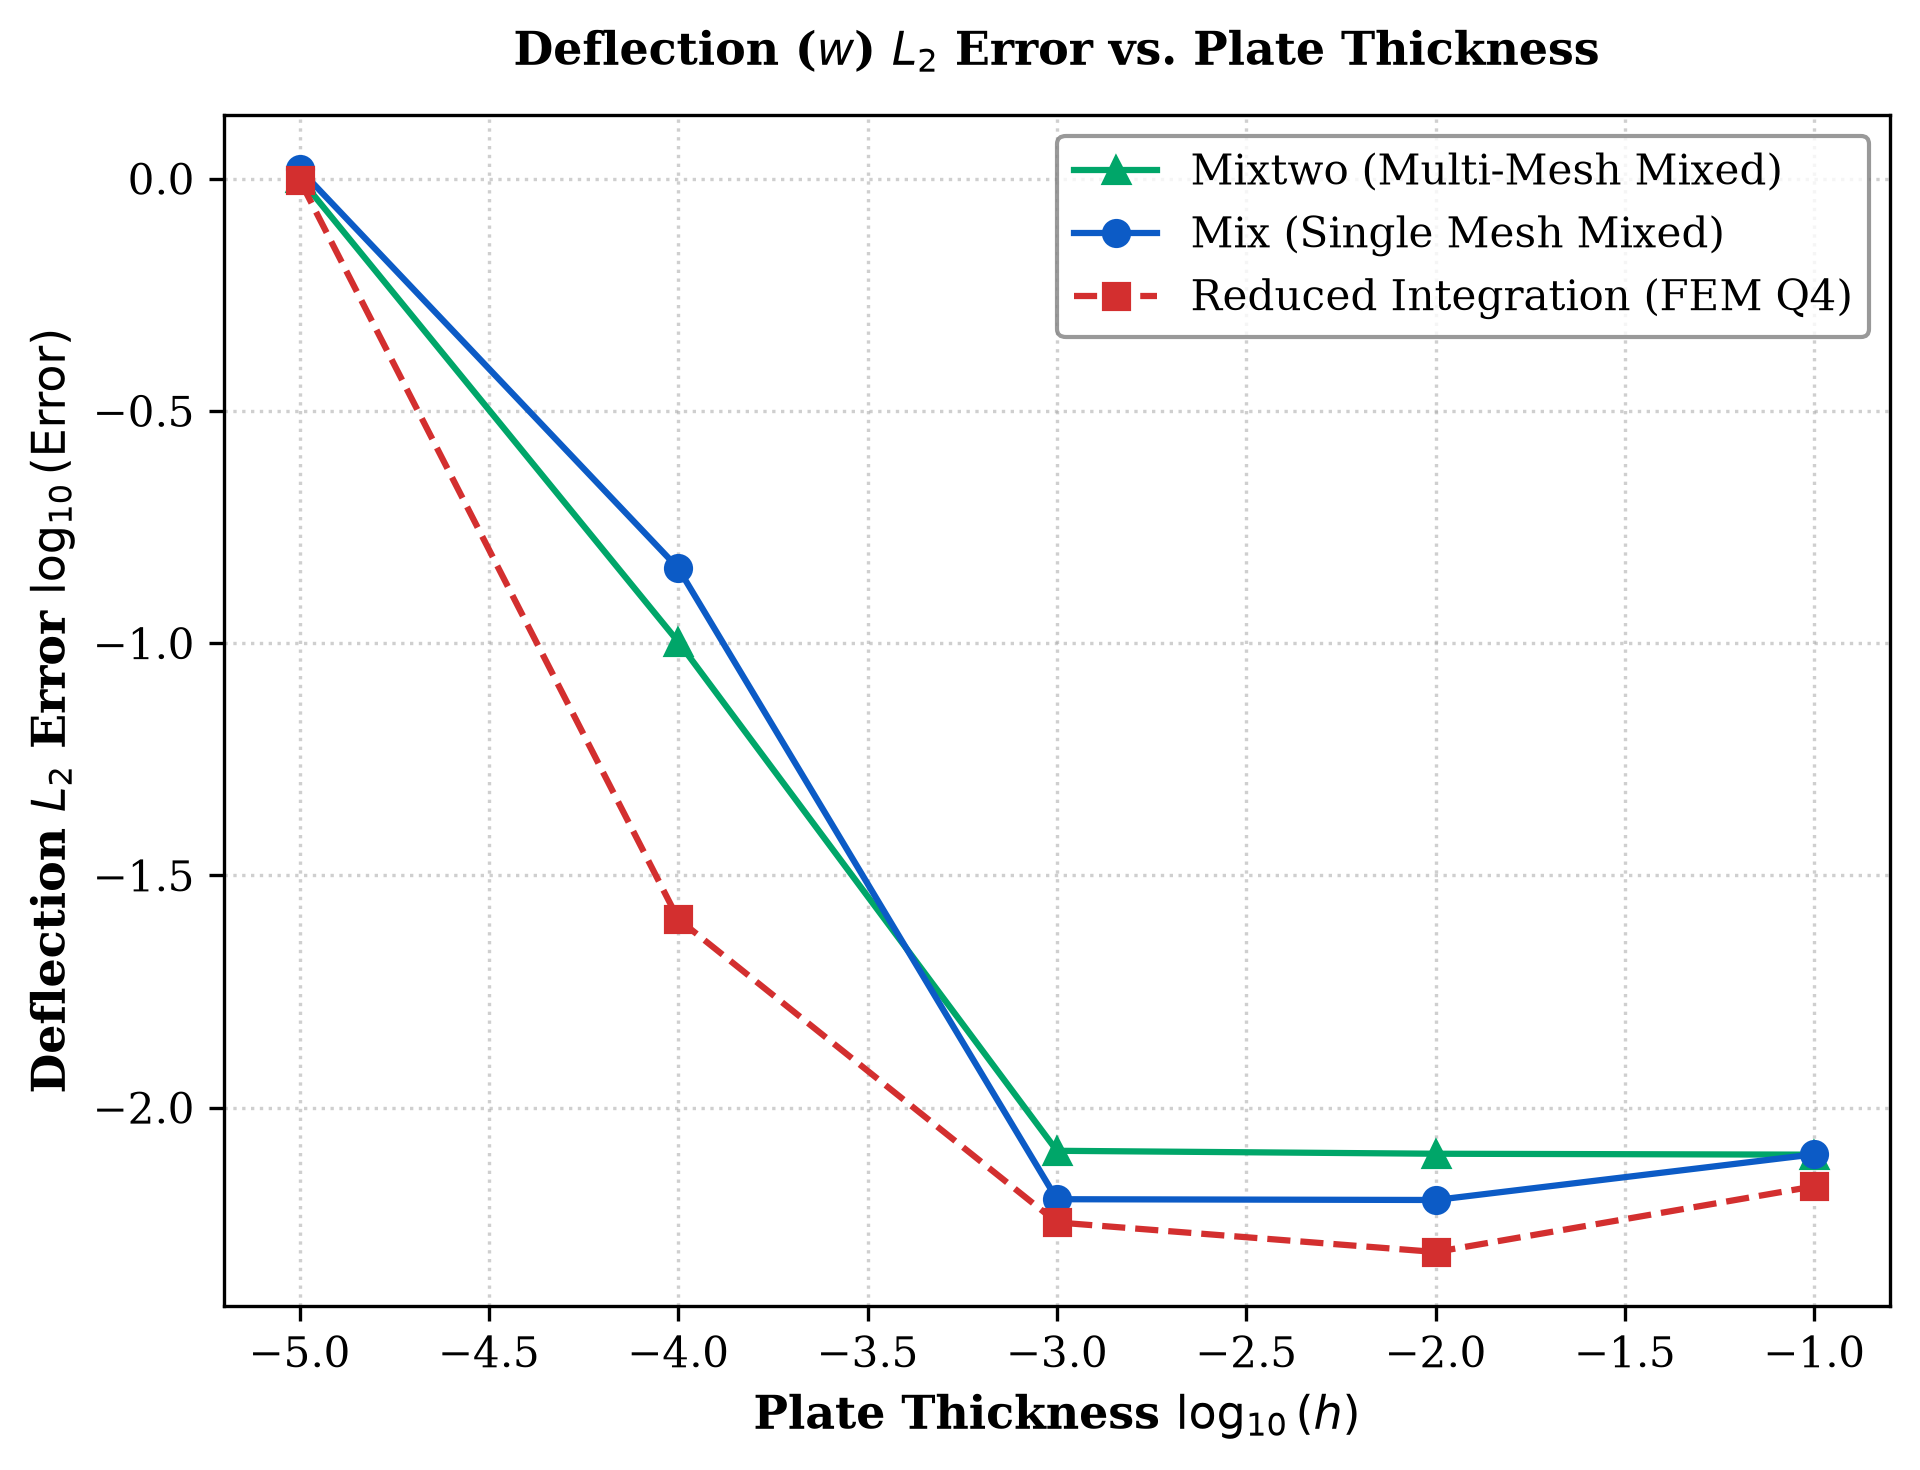
\includegraphics[width=0.6\textwidth]{vibration_thickness_w_convergence.png}
\caption{位移場（$w$）$L_2$ 誤差隨幾何厚度縮減之響應折線}
\label{fig:exp2_w}
\end{figure}

在位移場全域殘差測試中（圖~\ref{fig:exp2_w}），傳統有限元（紅線）在薄板極限區間無法展現幾何收斂，殘差直接在高位死線平盤橫變。而藍線（Mix）與綠線（Mixtwo）在全幾何跨度下，其位移 $L_2$ 殘差不升反降，全線維持在低水平區間穩定延伸，未受數值鎖死干擾。

\begin{figure}[h]
\centering
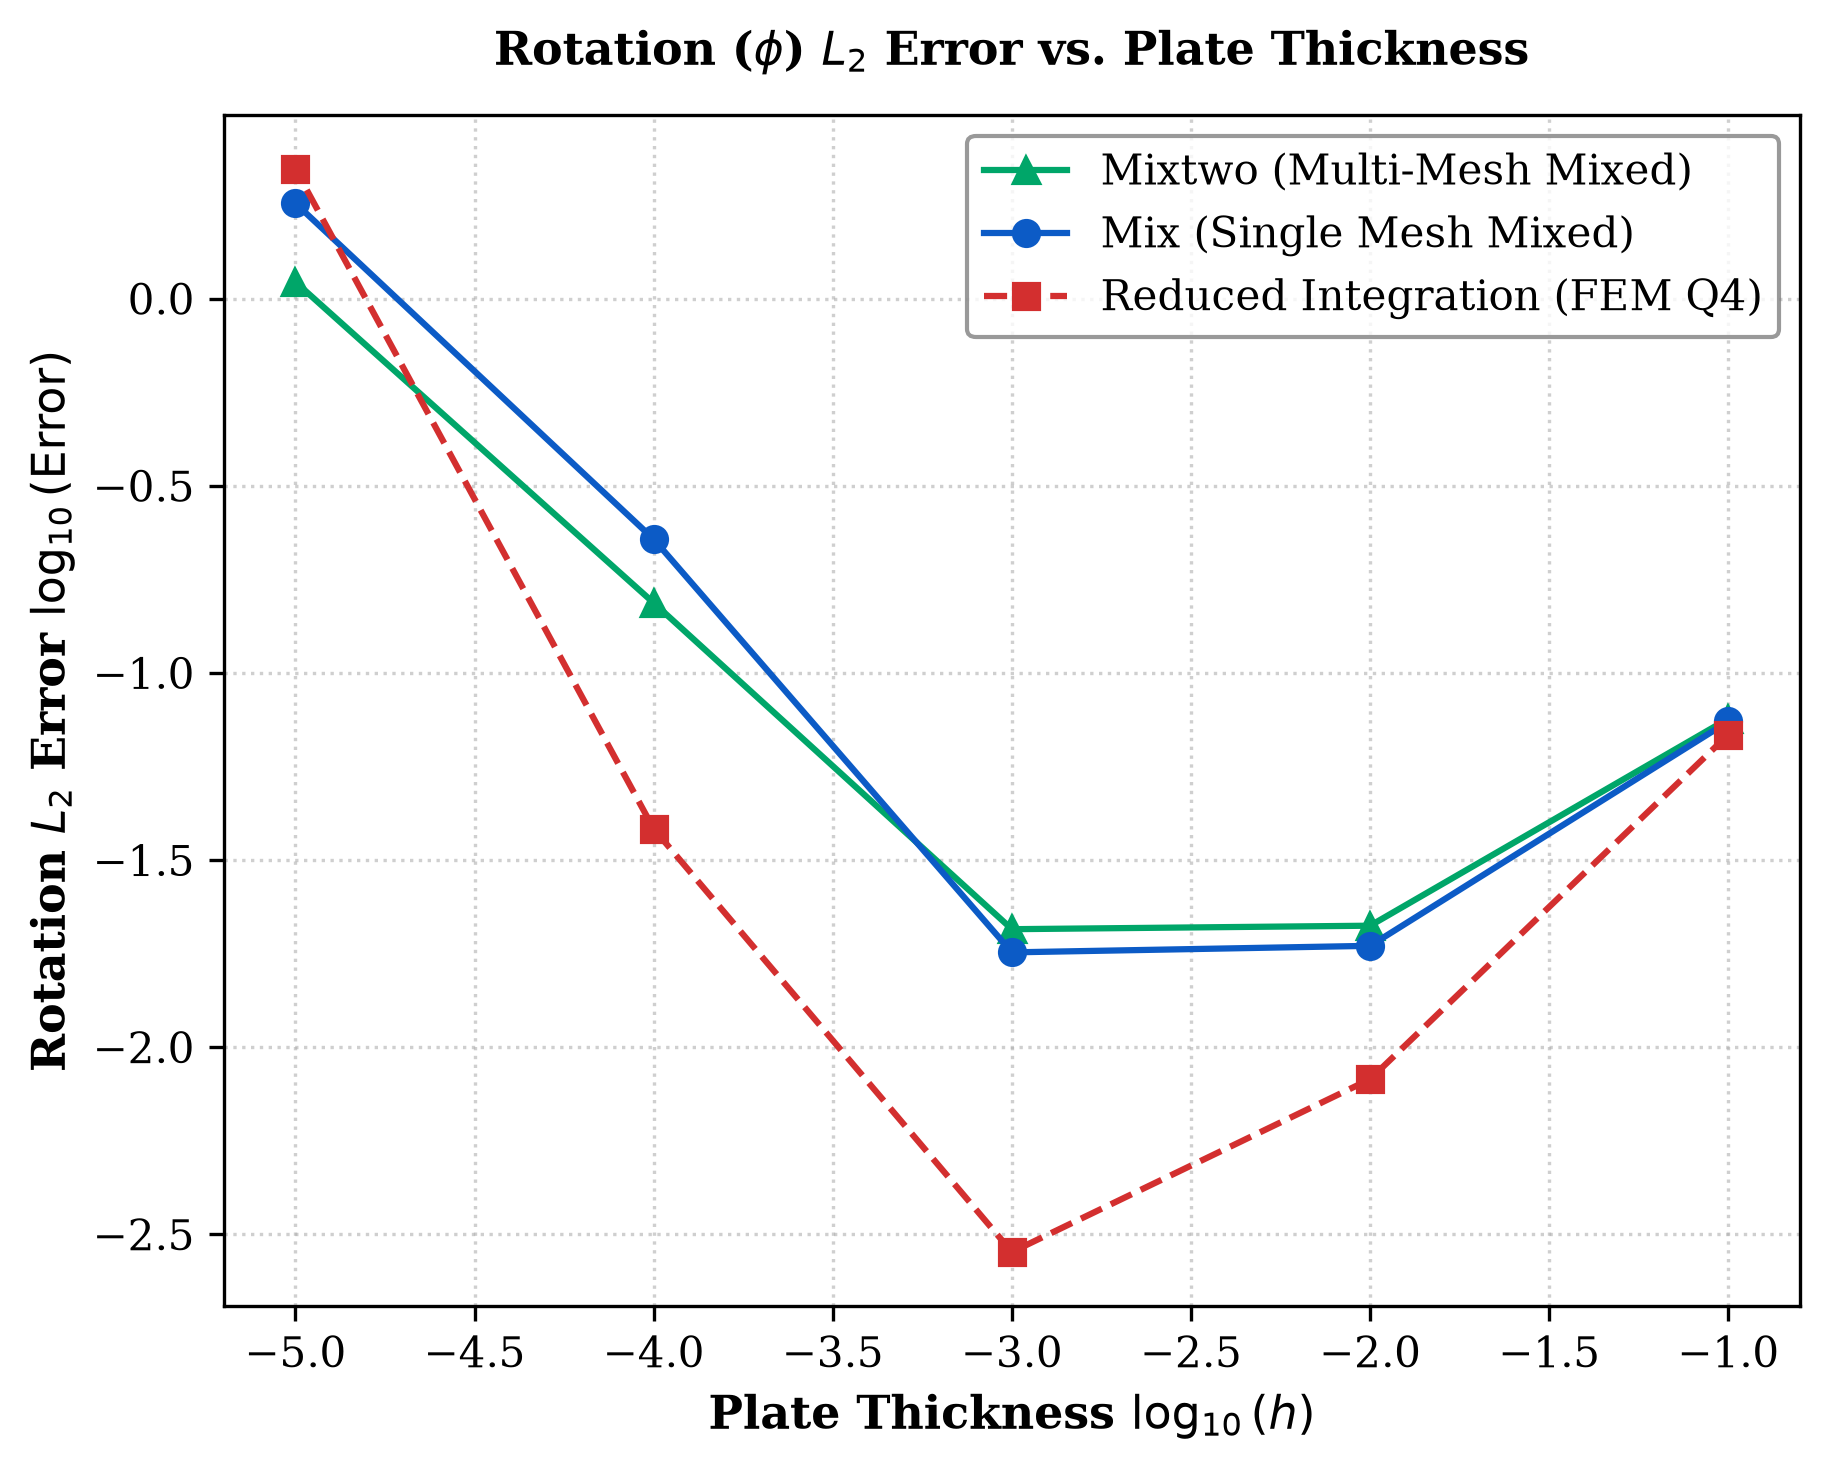
\includegraphics[width=0.6\textwidth]{vibration_thickness_phi_convergence.png}
\caption{轉角場（$\phi$）$L_2$ 誤差隨幾何厚度縮減之響應折線}
\label{fig:exp2_phi}
\end{figure}

如圖~\ref{fig:exp2_phi}~所示，轉角場的幾何殘差展現出與位移場高度一致的力學規律。傳統有限元（紅線）在超薄區域誤差擴大，而基於無網格重構核與多場混合變分的 Mix 與 Mixtwo 流派，在全域厚度範圍內皆表現出極佳的數值穩定性與力學正確性。

\end{document}